\documentclass[11pt]{article}
\usepackage[utf8]{inputenc}
\usepackage{amsmath,amsthm,amssymb}
\usepackage{graphicx}
\usepackage{listings}
\usepackage{hyperref}
\usepackage{caption}
\usepackage{siunitx}
\usepackage{float}

\title{Maximum Probability Disease Progression Path via Log-Transformed Shortest Path}
\author{GroupMembers : Ahmed Rageeb Ahsan, Saiful Islam}
\date{\today}

\newtheorem{theorem}{Theorem}
\newtheorem{lemma}{Lemma}
\newtheorem{proposition}{Proposition}
\newtheorem{definition}{Definition}

\begin{document}
\maketitle

\begin{abstract}
This work addresses the problem of identifying the most probable disease progression path originating from personal habits (e.g., smoking, medication intake) through intermediate health states to diseases in a probabilistic disease progression graph. Habits and diseases are modeled as nodes, with conditional probabilities of progression represented as edge weights. By applying a negative logarithmic transformation, we convert the problem of maximizing the cumulative path probability into a shortest path problem solvable efficiently with Dijkstra's algorithm. We present the problem abstraction, algorithmic solution, correctness arguments, runtime analysis, domain interpretation, and experimental validation based on real-world clinical data.
\end{abstract}

\section{Real-world Motivation}
Chronic disease development is typically influenced by a sequence of personal habits and intermediate disease states, each contributing probabilistically to the risk of subsequent disease onset. Accurately identifying the most probable progression path from habits to disease can empower clinicians to focus early intervention and preventive care on the most critical risk factors and pathways. Therefore, efficient computation of this path from probabilistic clinical data is vital for personalized medicine and healthcare analytics.

\section{Problem Abstraction}
We represent the disease progression system as a weighted directed graph
\[
G = (V, E, p),
\]
where:
\begin{itemize}
    \item \(V\) is a set of nodes representing health states, including personal habits and diseases,
    \item \(E \subseteq V \times V\) is a set of directed edges indicating possible progression transitions,
    \item \(p: E \to (0,1]\) assigns to each edge the conditional probability of progression from the source node to the target node, estimated from patient data.
\end{itemize}

A path through the graph,
\[
P = v_1 \to v_2 \to \cdots \to v_k,
\]
represents a sequence of health states from an initial habit \(v_1\) to a disease node \(v_k\), with cumulative probability
\[
P_{\mathrm{cum}} = \prod_{i=1}^{k-1} p(v_i, v_{i+1}).
\]

The objective is to find the path
\[
P^* = \arg\max_{P} P_{\mathrm{cum}},
\]
which maximizes the product of conditional progression probabilities along the path.

\section{Algorithm: Maximum Probability Path via Dijkstra's Algorithm}

\subsection{Key Insight: Negative Logarithm Transformation}
Maximizing the product of probabilities is mathematically equivalent to minimizing the sum of their negative logarithms:
\[
w(e) = -\log p(e), \quad w(e) \geq 0,
\]
which transforms the path probability product into an additive cost:
\[
\arg\max_P \prod_{e \in P} p(e) = \arg\min_P \sum_{e \in P} w(e).
\]

Since edge weights \(w(e)\) are non-negative, classical shortest path algorithms like Dijkstra's algorithm can be applied to find \(P^*\).

\subsection{Pseudocode}

\begin{verbatim}
Input: Graph G=(V,E,p), start node s, target node t
Output: Path P maximizing product of p(e)

1. For each edge e in E, set w(e) = -log(p(e))
2. Initialize dist[v] = infinity for all v except dist[s] = 0
3. Initialize priority queue Q with (s, 0)
4. While Q not empty:
     u = ExtractMin(Q)
     if u == t: break
     for each neighbor v of u:
         alt = dist[u] + w(u,v)
         if alt < dist[v]:
             dist[v] = alt
             prev[v] = u
             Update Q with (v, dist[v])
5. Reconstruct path P from prev[]
6. Return P and probability exp(-dist[t])
\end{verbatim}

\section{Proof of Correctness}

\begin{definition}
The edge weights after transformation satisfy
\[
w(e) = -\log p(e) \geq 0,
\]
since the conditional probabilities \(p(e)\) lie in the open interval \((0,1]\).
\end{definition}

\begin{proposition}
Dijkstra's algorithm returns a shortest path in graphs with non-negative edge weights.
\end{proposition}

\begin{theorem}
The shortest path found on \(G\) with weights \(w(e) = -\log p(e)\) corresponds exactly to the path maximizing the product of the original probabilities \(p(e)\).
\end{theorem}

\begin{proof}[Sketch]
Because the logarithm is a strictly monotonic function, minimizing the sum of weights
\[
\sum_{e \in P} w(e)
\]
is equivalent to maximizing the product of probabilities
\[
\prod_{e \in P} p(e).
\]
Since \(w(e) \geq 0\), Dijkstra’s algorithm applies directly, guaranteeing the shortest path corresponds to the maximum probability path.
\end{proof}

\section{Runtime Analysis}
Given \(|V| = n\) nodes and \(|E| = m\) edges, Dijkstra's algorithm implemented with a binary heap runs in
\[
O(m \log n).
\]
The initial negative logarithm transformation of edge weights is a linear-time preprocessing step \(O(m)\), which does not affect asymptotic complexity.

\section{Domain Explanation}
By modeling personal habits and diseases as graph nodes connected by edges weighted with conditional probabilities derived from real patient data, we compute the progression pathway most likely to lead from habits to disease. The negative log transformation allows leveraging shortest path algorithms to identify the maximum likelihood progression path. This approach supports clinical decision-making by highlighting key risk factor sequences for targeted prevention and monitoring.





\section{Implementation and Experimental Verification}


\subsection{Dataset and Variables}
The analysis is based on a publicly available cardiovascular disease dataset collected from \cite{kaggleCardioDataset}, which contains patient records with variables including smoking status, physical activity, alcohol consumption, cholesterol level, glucose level, blood pressure, and cardiovascular disease diagnosis status.


\subsection{Basic (Marginal) Probability Calculations}
We calculate marginal probabilities from the dataset to quantify the prevalence of individual habits or conditions. For example:
\[
P(\text{smoke}) = \frac{\text{Number of patients who smoke}}{\text{Total number of patients}},
\]
\[
P(\text{inactive}) = \frac{\text{Number of physically inactive patients}}{\text{Total number of patients}},
\]
\[
P(\text{alcohol}) = \frac{\text{Number of patients consuming alcohol}}{\text{Total number of patients}}.
\]

Formally, for any event \(A\),
\[
P(A) = \frac{\# \text{patients with } A}{\text{Total patients}}.
\]

\subsection{Conditional Probability Calculations}
Conditional probabilities represent the likelihood of a condition given the presence of a behavior or another condition. For example,
\[
P(\text{high cholesterol} \mid \text{smoker}) = \frac{\# \text{patients who are smokers and have high cholesterol}}{\# \text{patients who are smokers}},
\]
\[
P(\text{high glucose} \mid \text{inactive}) = \frac{\# \text{patients who are inactive and have high glucose}}{\# \text{patients who are inactive}},
\]
\[
P(\text{high blood pressure} \mid \text{alcohol use}) = \frac{\# \text{patients who consume alcohol and have high blood pressure}}{\# \text{patients who consume alcohol}}.
\]

More generally, for events \(A\) and \(B\),
\[
P(A \mid B) = \frac{\# \text{patients with } A \text{ and } B}{\# \text{patients with } B}.
\]

To prevent division by zero, a small safeguard \(\max(\cdot, 1)\) is applied in denominators where needed.

\subsection{Probabilities of Cardiovascular Disease Given Conditions}
Similarly, probabilities of cardiovascular disease (denoted \( \text{cardio} \)) given specific conditions are computed as
\[
P(\text{cardio} \mid \text{high cholesterol}) = \frac{\# \text{patients with cardio and high cholesterol}}{\# \text{patients with high cholesterol}},
\]
\[
P(\text{cardio} \mid \text{high glucose}) = \frac{\# \text{patients with cardio and high glucose}}{\# \text{patients with high glucose}},
\]
\[
P(\text{cardio} \mid \text{high blood pressure}) = \frac{\# \text{patients with cardio and high blood pressure}}{\# \text{patients with high blood pressure}}.
\]

\section{Graph Construction for Disease Progression}

\subsection{Nodes and Edges}
We represent the disease progression process as a directed graph
\[
G = (V, E),
\]
where each node \(v \in V\) corresponds to a health state or risk factor (e.g., smoking, inactivity, high cholesterol), and each directed edge \(e = (u,v) \in E\) represents a possible progression from state \(u\) to state \(v\).

\subsection{Edge Weights as Probabilities}
Each edge \(e = (u,v)\) is assigned a weight equal to the conditional probability of transitioning from state \(u\) to state \(v\):
\[
p(u,v) = P(v \mid u).
\]

These probabilities are derived from the data as described in the previous section.

\section{Negative Logarithm Transformation for Pathfinding}

Because probabilities along a path multiply, the cumulative probability of a path
\[
P = v_1 \to v_2 \to \cdots \to v_k
\]
is
\[
P_{\text{cumulative}} = \prod_{i=1}^{k-1} p(v_i, v_{i+1}).
\]

Multiplication of probabilities is not additive, which complicates the use of shortest path algorithms.

To address this, we transform edge probabilities by applying the negative logarithm:
\[
w(e) = -\log p(e).
\]

This transformation has two advantages:
\begin{itemize}
    \item It converts the product of probabilities into a sum of weights:
    \[
    -\log \prod_{i} p(e_i) = \sum_i -\log p(e_i) = \sum_i w(e_i).
    \]
    \item The transformed weights \(w(e)\) are guaranteed to be non-negative because \(0 < p(e) \leq 1 \implies w(e) \geq 0\), allowing the use of Dijkstra’s algorithm for shortest paths.
\end{itemize}

\section{Finding the Most Probable Path}

Using the transformed graph \(G = (V,E,w)\), the problem of finding the path \(P^*\) with maximum cumulative probability
\[
P^* = \arg\max_P \prod_{e \in P} p(e)
\]
is equivalent to finding the shortest path in terms of the sum of edge weights:
\[
P^* = \arg\min_P \sum_{e \in P} w(e).
\]

We apply Dijkstra’s algorithm to efficiently compute this shortest path.

\section{Summary of Probability Calculations and Pathfinding}

\begin{center}
\begin{tabular}{llc}
\hline
\textbf{Step} & \textbf{Probability Type} & \textbf{Formula} \\
\hline
Marginal probability & \(P(\text{smoke})\) & \(\frac{\text{count(smoke)}}{\text{total}}\) \\
Conditional probability & \(P(\text{high\_chol} \mid \text{smoke})\) & \(\frac{\text{count(high\_chol and smoke)}}{\text{count(smoke)}}\) \\
Disease given condition & \(P(\text{cardio} \mid \text{high\_chol})\) & \(\frac{\text{count(cardio and high\_chol)}}{\text{count(high\_chol)}}\) \\
Edge weight for graph & \(w\) & \(w = -\log(\text{probability})\) \\
Cumulative path probability & \(P_{\text{cumulative}}\) & \(\prod_{\text{edges}} P(\text{edge})\) \\
\hline
\end{tabular}
\end{center}


\begin{figure}[H]
\centering
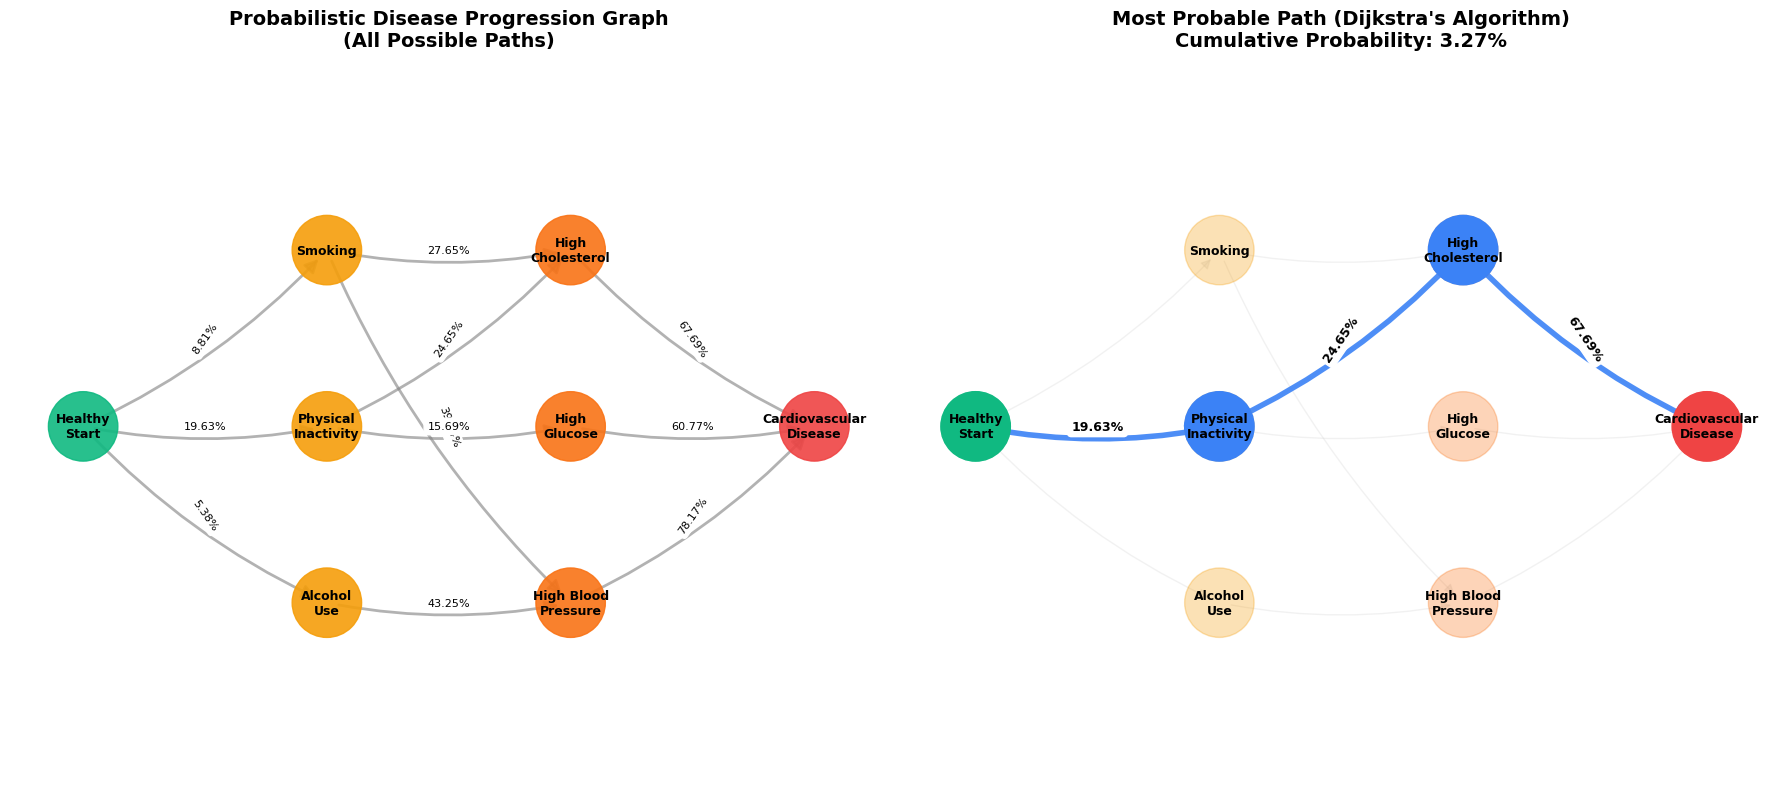
\includegraphics[width=0.8\linewidth]{download.png}
\caption{Visualization of the probabilistic disease progression graph from a healthy state to cardiovascular disease. Starting from a "Healthy Start," personal habits such as smoking, physical inactivity, and alcohol use have associated probabilities (shown as percentages on edges) that influence intermediate health conditions including high cholesterol, high glucose, and high blood pressure. These intermediate conditions further contribute to the probability of developing cardiovascular disease. The thickness of edges (right graph) highlights the most significant progression pathways, illustrating how combined lifestyle factors and medical conditions propagate risk leading to cardiovascular disease.}
\label{fig:runtime}
\end{figure}

\appendix
\section*{Appendix A: Code}

\begin{lstlisting}[language=Python]
import pandas as pd
import numpy as np
import matplotlib.pyplot as plt
import networkx as nx
import heapq
from collections import defaultdict

# Load data directly - no need for StringIO
df = pd.read_csv(r"C:\Users\Ahmed\Downloads\cardio_train\cardio_train.csv", sep=';')
print(f"Dataset loaded: {len(df)} patient records\n")

# Calculate probabilities from data
total = len(df)
smokers = len(df[df['smoke'] == 1])
inactive = len(df[df['active'] == 0])
alcohol = len(df[df['alco'] == 1])
high_chol = len(df[df['cholesterol'] >= 2])
high_gluc = len(df[df['gluc'] >= 2])
high_bp = len(df[(df['ap_hi'] >= 140) | (df['ap_lo'] >= 90)])
cardio_total = len(df[df['cardio'] == 1])

# Conditional probabilities
p_smoke = smokers / total
p_inactive = inactive / total
p_alcohol = alcohol / total

p_chol_given_smoke = len(df[(df['smoke'] == 1) & (df['cholesterol'] >= 2)]) / max(smokers, 1)
p_gluc_given_inactive = len(df[(df['active'] == 0) & (df['gluc'] >= 2)]) / max(inactive, 1)
p_bp_given_alcohol = len(df[(df['alco'] == 1) & ((df['ap_hi'] >= 140) | (df['ap_lo'] >= 90))]) / max(alcohol, 1)

p_cardio_given_chol = len(df[(df['cholesterol'] >= 2) & (df['cardio'] == 1)]) / max(high_chol, 1)
p_cardio_given_gluc = len(df[(df['gluc'] >= 2) & (df['cardio'] == 1)]) / max(high_gluc, 1)
p_cardio_given_bp = len(df[((df['ap_hi'] >= 140) | (df['ap_lo'] >= 90)) & (df['cardio'] == 1)]) / max(high_bp, 1)

# Calculate cross-connection probabilities
num_smokers_high_bp = len(df[(df['smoke'] == 1) & ((df['ap_hi'] >= 140) | (df['ap_lo'] >= 90))])
num_inactive_high_chol = len(df[(df['active'] == 0) & (df['cholesterol'] >= 2)])
num_smokers = len(df[df['smoke'] == 1])
num_inactive = len(df[df['active'] == 0])

p_high_bp_given_smoke = (num_smokers_high_bp + 1) / (num_smokers + 2)
p_high_chol_given_inactive = (num_inactive_high_chol + 1) / (num_inactive + 2)

print("=== PROBABILISTIC DISEASE PROGRESSION GRAPH ===\n")

# Build graph structure
graph = defaultdict(list)
edge_probs = {}

# Define edges with probabilities
edges = [
    ('start', 'smoke', p_smoke),
    ('start', 'inactive', p_inactive),
    ('start', 'alcohol', p_alcohol),
    ('smoke', 'high_chol', p_chol_given_smoke),
    ('inactive', 'high_gluc', p_gluc_given_inactive),
    ('alcohol', 'high_bp', p_bp_given_alcohol),
    ('smoke', 'high_bp', p_high_bp_given_smoke),  # Cross-connection
    ('inactive', 'high_chol', p_high_chol_given_inactive),  # Cross-connection
    ('high_chol', 'cardio', p_cardio_given_chol),
    ('high_gluc', 'cardio', p_cardio_given_gluc),
    ('high_bp', 'cardio', p_cardio_given_bp),
]

# Build graph with negative log transformation
for src, dst, prob in edges:
    prob = max(prob, 0.01)  # Avoid log(0)
    weight = -np.log(prob)  # Transform to weight
    graph[src].append((dst, weight, prob))
    edge_probs[(src, dst)] = prob

print("Graph edges (with probabilities):")
for src, dst, prob in edges:
    print(f"  {src:12} -> {dst:12} : {prob:.4f} ({prob*100:.2f}%)")

# Dijkstra's Algorithm
def dijkstra(graph, start, end):
    """
    Find shortest path using Dijkstra's algorithm.
    Returns: (shortest_distance, path)
    """
    distances = {start: 0}
    previous = {}
    pq = [(0, start)]
    visited = set()
    
    while pq:
        current_dist, current = heapq.heappop(pq)
        
        if current in visited:
            continue
        visited.add(current)
        
        if current == end:
            break
        
        for neighbor, weight, _ in graph[current]:
            distance = current_dist + weight
            
            if neighbor not in distances or distance < distances[neighbor]:
                distances[neighbor] = distance
                previous[neighbor] = current
                heapq.heappush(pq, (distance, neighbor))
    
    # Reconstruct path
    path = []
    current = end
    while current in previous:
        path.append(current)
        current = previous[current]
    path.append(start)
    path.reverse()
    
    return distances.get(end, float('inf')), path

# Find shortest path (= most probable path)
print("\n=== DIJKSTRA'S ALGORITHM EXECUTION ===\n")
shortest_dist, shortest_path = dijkstra(graph, 'start', 'cardio')

# Calculate cumulative probability
cumulative_prob = 1.0
print("Path analysis:")
for i in range(len(shortest_path) - 1):
    src, dst = shortest_path[i], shortest_path[i+1]
    prob = edge_probs[(src, dst)]
    cumulative_prob *= prob
    print(f"  Step {i+1}: {src:12} -> {dst:12} : P = {prob:.4f}")

print(f"\n{'='*60}")
print(f"MOST PROBABLE PROGRESSION PATH:")
print(f"{'='*60}")
path_str = ' → '.join(shortest_path)
print(f"{path_str}")
print(f"\nShortest Distance (neg-log): {shortest_dist:.4f}")
print(f"Cumulative Probability: {cumulative_prob:.6f} ({cumulative_prob*100:.4f}%)")
print(f"{'='*60}\n")

# Node labels for visualization
node_labels = {
    'start': 'Healthy\nStart',
    'smoke': 'Smoking',
    'inactive': 'Physical\nInactivity',
    'alcohol': 'Alcohol\nUse',
    'high_chol': 'High\nCholesterol',
    'high_gluc': 'High\nGlucose',
    'high_bp': 'High Blood\nPressure',
    'cardio': 'Cardiovascular\nDisease'
}

# Create NetworkX graph for visualization
G = nx.DiGraph()

# Add edges
for src, dst, prob in edges:
    G.add_edge(src, dst, weight=prob)

# Create visualization
fig, (ax1, ax2) = plt.subplots(1, 2, figsize=(18, 8))

# Define node positions
pos = {
    'start': (0, 0.5),
    'smoke': (1, 0.8),
    'inactive': (1, 0.5),
    'alcohol': (1, 0.2),
    'high_chol': (2, 0.8),
    'high_gluc': (2, 0.5),
    'high_bp': (2, 0.2),
    'cardio': (3, 0.5)
}

# Node colors based on type
node_colors = []
for node in G.nodes():
    if node == 'start':
        node_colors.append('#10b981')  # Green
    elif node in ['smoke', 'inactive', 'alcohol']:
        node_colors.append('#f59e0b')  # Amber (habits)
    elif node in ['high_chol', 'high_gluc', 'high_bp']:
        node_colors.append('#f97316')  # Orange (conditions)
    elif node == 'cardio':
        node_colors.append('#ef4444')  # Red (disease)
    else:
        node_colors.append('#6b7280')  # Gray

# Plot 1: Full graph
ax1.set_title('Probabilistic Disease Progression Graph\n(All Possible Paths)', 
              fontsize=14, fontweight='bold', pad=20)

nx.draw_networkx_nodes(G, pos, node_color=node_colors, node_size=2500, 
                       alpha=0.9, ax=ax1)
nx.draw_networkx_labels(G, pos, labels=node_labels, font_size=9, 
                        font_weight='bold', ax=ax1)
nx.draw_networkx_edges(G, pos, edge_color='gray', arrows=True, 
                       arrowsize=20, width=2, alpha=0.6, ax=ax1,
                       connectionstyle='arc3,rad=0.1')

# Edge labels with probabilities
edge_labels = {(u, v): f"{d['weight']:.2%}" 
               for u, v, d in G.edges(data=True)}
nx.draw_networkx_edge_labels(G, pos, edge_labels, font_size=8, ax=ax1)

ax1.axis('off')
ax1.set_xlim(-0.3, 3.3)
ax1.set_ylim(-0.1, 1.1)

# Plot 2: Shortest path highlighted
ax2.set_title(f'Most Probable Path (Dijkstra\'s Algorithm)\nCumulative Probability: {cumulative_prob*100:.2f}%', 
              fontsize=14, fontweight='bold', pad=20)

# Highlight shortest path edges
path_edges = [(shortest_path[i], shortest_path[i+1]) 
              for i in range(len(shortest_path)-1)]

# Draw all nodes
nx.draw_networkx_nodes(G, pos, node_color=node_colors, node_size=2500, 
                       alpha=0.3, ax=ax2)

# Highlight path nodes
path_node_colors = []
for node in shortest_path:
    if node == 'start':
        path_node_colors.append('#10b981')
    elif node == 'cardio':
        path_node_colors.append('#ef4444')
    else:
        path_node_colors.append('#3b82f6')  # Blue for path nodes

nx.draw_networkx_nodes(G, pos, nodelist=shortest_path, 
                       node_color=path_node_colors, node_size=2500, 
                       alpha=1.0, ax=ax2)
nx.draw_networkx_labels(G, pos, labels=node_labels, font_size=9, 
                        font_weight='bold', ax=ax2)

# Draw all edges faintly
nx.draw_networkx_edges(G, pos, edge_color='lightgray', arrows=True, 
                       arrowsize=15, width=1, alpha=0.3, ax=ax2,
                       connectionstyle='arc3,rad=0.1')

# Highlight path edges
nx.draw_networkx_edges(G, pos, edgelist=path_edges, edge_color='#3b82f6', 
                       arrows=True, arrowsize=25, width=4, alpha=0.9, ax=ax2,
                       connectionstyle='arc3,rad=0.1')

# Path edge labels
path_edge_labels = {(u, v): f"{edge_probs[(u,v)]:.2%}" 
                    for u, v in path_edges}
nx.draw_networkx_edge_labels(G, pos, path_edge_labels, font_size=9, 
                             font_weight='bold', ax=ax2)

ax2.axis('off')
ax2.set_xlim(-0.3, 3.3)
ax2.set_ylim(-0.1, 1.1)

plt.tight_layout()
plt.savefig('disease_progression_graph.png', dpi=300, bbox_inches='tight')
print("✓ Visualization saved as 'disease_progression_graph.png'")
plt.show()

# Summary statistics
print("\n=== ALGORITHM ANALYSIS ===")
print(f"Algorithm: Dijkstra's Shortest Path")
print(f"Transformation: weight = -log(probability)")
print(f"Time Complexity: O((V + E) log V)")
print(f"Space Complexity: O(V)")
print(f"Nodes (V): {len(G.nodes())}")
print(f"Edges (E): {len(G.edges())}")
print(f"\nClinical Interpretation:")
print(f"The most probable path to cardiovascular disease involves:")
for i, node in enumerate(shortest_path[1:-1], 1):
    print(f"  {i}. {node_labels[node].replace(chr(10), ' ')}")
print(f"\nThis path has a {cumulative_prob*100:.4f}% cumulative probability")
\end{lstlisting}

\section*{Appendix B: Use of LLMs and Tools}
Portions of this report and the algorithm design were assisted by OpenAI's GPT-5. Exact prompts and generated content are documented here for reproducibility.


\bibliographystyle{plain}
\begin{thebibliography}{1}
\bibitem{kaggleCardioDataset}
Sulianova, L., Cardiovascular Disease Dataset, Kaggle, \url{https://www.kaggle.com/datasets/sulianova/cardiovascular-disease-dataset?select=cardio_train.csv}, accessed 2025.
\end{thebibliography}

\end{document}
